\section{Evaluation}
\label{sec:method}
%
\subsection{Methodology}

\niparagraph{Baseline.}
%
For evaluation, we compare three baseline systems along with our \neupims system, namely GPU-only, NPU-only, and NPU+PIM.
%
\begin{itemize}[labelindent=0.1em,nolistsep,leftmargin=1em]
    \item \textbf{\textsf{GPU-only}:}
    %
    \textsf{GPU-only} is a real GPU system. We conduct experiments with an A100 40GB GPU, and we compile the LLM batched inference workload with PyTorch~\cite{pytorch}.
    
    \item \textbf{NPU-only:}
    %
    NPU-only represents existing NPU accelerators such as TPU, without any PIM capabilities. 
    %
    We assume that this baseline has the equivalent memory bandwidth with other alternatives for fairness. 
    %
    Moreover, a NPU is equipped with not only systolic array but also GPU-like vector processing units to support \emph{non}-GEMM operators.  
    %
    \item \textbf{NPU+PIM:}
    %
    NPU+PIM is also a PIM-enabled NPU baseline, which integrates existing PIM-based GEMV accelerators~\cite{newton} with the off-the-shelf NPU accelerator. 
    %
    We merely map the GEMV operations in MHA layers to the PIM, while all the others are computed at the NPU side.
    %
    We allocate the requests to PIM channels in a round-robin manner.
    %
\end{itemize}

\niparagraph{Cycle-level simulation.}
We build the \neupims simulator on two open-source cycle-accurate simulators, ONNXim~\cite{onnxim} and DRAMsim3~\cite{dramsim3}. 
%
We link the two simulators by modifying the memory interface of ONNXim and offloading the memory accesses to the PIM simulator based on DRAMsim3.
%

\begin{table}[]
\caption{\neupims hardware specification.}
\footnotesize
\vspace{-2ex}
\label{tab:hardware-spec}
\begin{tabular}{cccc}
\hline
\multicolumn{2}{c|}{\textbf{NPU Configuration}}                                                         & \multicolumn{2}{c}{\textbf{HBM Organization}}                             \\ \hline
\multicolumn{1}{c|}{Systolic Arrays/Chip}                & \multicolumn{1}{c|}{8}                       & \multicolumn{1}{c|}{Banks/Bankgroup}                 & 4                  \\
\multicolumn{1}{c|}{Vector Units/Chip}                   & \multicolumn{1}{c|}{8}                       & \multicolumn{1}{c|}{Banks/Channel}                   & 32                 \\
\multicolumn{1}{c|}{HBM Channels/Chip}                   & \multicolumn{1}{c|}{32}                      & \multicolumn{1}{c|}{Frequency}                           & 1GHz               \\
\multicolumn{1}{c|}{Systolic Array Size}                 & \multicolumn{1}{c|}{128 x 128}               & \multicolumn{1}{c|}{Capacity/Channel}                & 1GB                \\
\multicolumn{1}{c|}{Vector Unit Size}                    & \multicolumn{1}{c|}{128 x 1}               & \multicolumn{1}{c|}{Page Size}                       & 1KB                \\ \hline
\multicolumn{4}{c}{\textbf{HBM Timing Parameter}}                                                                                                                                   \\ \hline
\multicolumn{4}{c}{\begin{tabular}[c]{@{}c@{}}tRP = 14, tRCD = 14, tRAS = 34, tRRD\_L = 6, tWR = 16, \\ tCCD\_S = 1, tCCD\_L = 2, tREFI = 3900, tRFC = 260, tFAW = 30\end{tabular}} \\ \hline
\end{tabular}
\vspace{-2ex}
\end{table}
%
\niparagraph{Hardware specifications.}
%
We prototype \neupims accelerator using a set of hardware specifications, which are listed in Table~\ref{tab:hardware-spec}.
%
Our \neupims accelerator prototype is a multi-chiplet design containing 8 systolic arrays, each integrated with a SIMD vector unit that serves activation operations.
%
Each memory channel controls 32 PIM banks, which offer in aggregate 1GB memory capacity. 
%
Note that while we choose this set of specifications for prototyping purposes, the \neupims architecture is orthogonal to these choices, allowing varying configurations depending on the model size and data-specific properties (e.g., sequence lengths). 

\begin{figure*}[t]
        \centering
        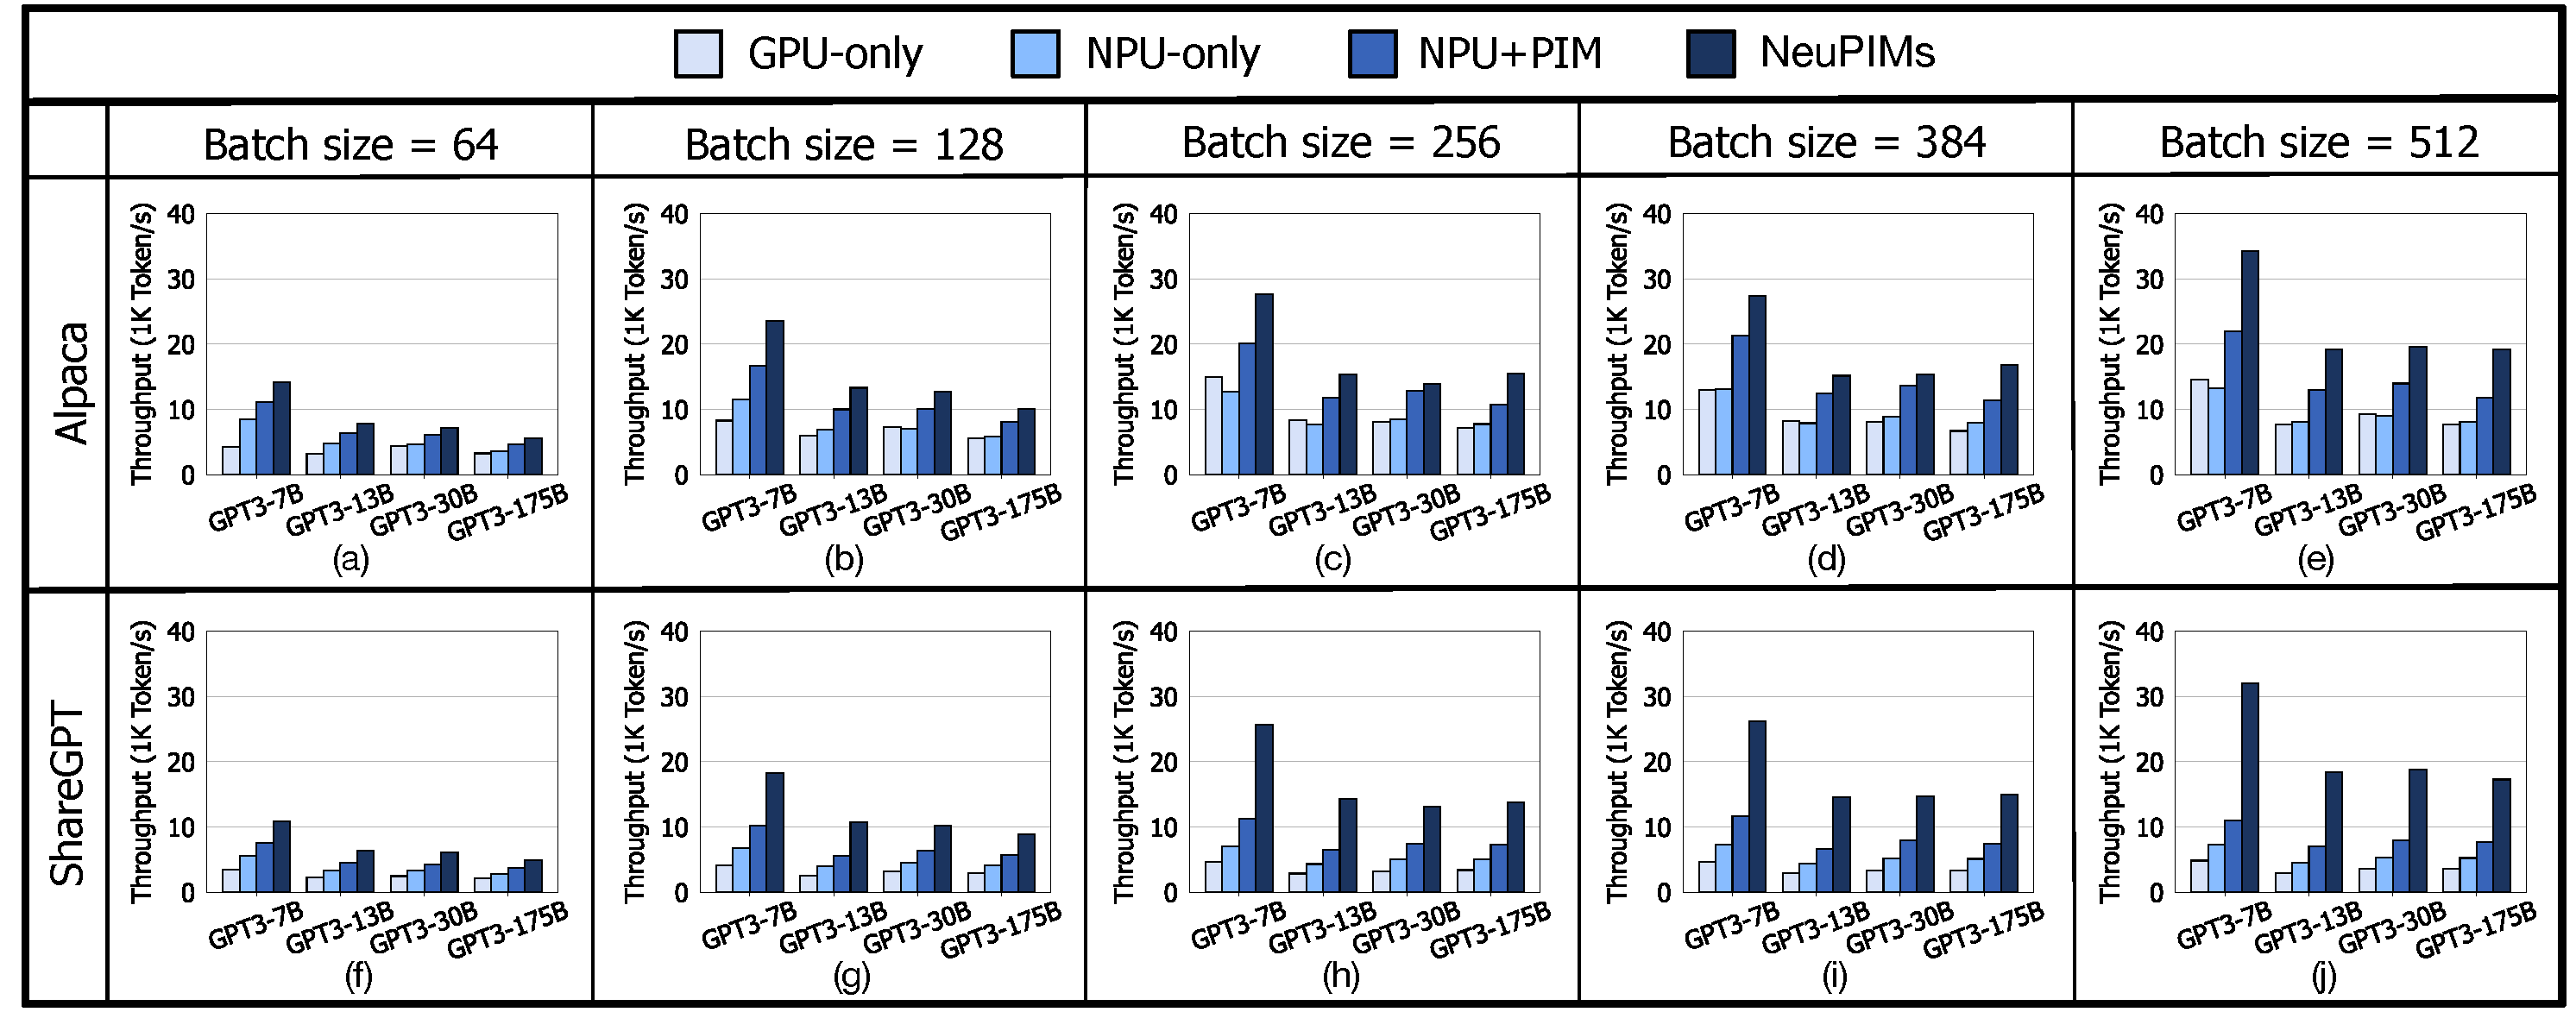
\includegraphics[width=1\linewidth]{figure/eval-throughput.pdf}
        \vspace{-2ex}
        \caption{Throughput comparison results of GPU-only, NPU-only, NPU+PIM, and \neupims. We use the two datasets, (a) Alpaca and (b) ShareGPT, using the batch sizes including 64, 128, 256, 384, and 512.}
        \vspace{-2ex}
        \label{fig:eval-end-to-end}
\end{figure*}

\begin{table}[]
\renewcommand{\arraystretch}{1.1}
\centering
\caption{The evaluated LLM configurations.}
\vspace{-2ex}
\label{tab:model-config}
\footnotesize
\begin{tabular}{c|ccc|cc}
\hline
\textbf{Model}     
& \textbf{$\#$ Layers}
& \textbf{$\#$ Heads}
& \textbf{d$_{model}$}
& \textbf{\# TP}
& \textbf{\# PP}
\\ \hline

GPT3-7B & 32 & 32 & 4096 & 4 & 1 \\
GPT3-13B  & 40 & 40 & 5120 & 4 & 1 \\
GPT3-30B  & 48 & 56 & 7168 & 4 & 2 \\
GPT3-175B & 96 & 96 & 12288 & 8 & 4 \\ 
\hline
\end{tabular}
\vspace{-2ex}
\end{table}

% %
\niparagraph{LLM models.}
%
We use four variants of GPT3, a state-of-the-art LLM developed by OpenAI as described in Table~\ref{tab:model-config}.
%
While our experiments focus on GPT-3 model variants, \neupims can host any decoder-based generation models, offering generality and wide applicability. 
%

\niparagraph{Datasets.}
%
We use two real-world LLM inferencing datasets, ShareGPT~\cite{sharegpt} and Alpaca~\cite{alpaca}. 
%
ShareGPT dataset is a set of conversations scraped from the real-world user log of ChatGPT~\cite{openai-chatgpt}. 
%
Alpaca dataset is an instruction dataset generated by OpenAI's text-davinci-003 engine. 
%
The two datasets have distributions for input and output sequences. 
%
ShareGPT has an average input token length of 80 and an output of 296, while Alpaca has shorter sequence lengths of 12 and 56 for input and output, respectively.

%
\niparagraph{Workload.}
%
As running experiments for inference serving scenarios with a cycle-accurate simulator is infeasible, we develop an alternative methodology to synthesize workloads for system-level evaluation. 
%
To define the search space for workloads, we consider various hyperparameters, including model types, batch sizes, and tensor/pipeline parallelism.
%
For each permutation of these hyperparameters, we simulate the inference serving for a fixed amount of time, randomly picking sequence lengths from the datasets. 
%
This way, we can warm up the inference batch in a way that the batch is filled with requests having various sequence lengths. 
%
We sample 10 different batches and use them to measure the throughputs of different hyperparameter combinations.
%